\documentclass{main}
%----------------------------------------------------------------------------------------
%	Definitions
%----------------------------------------------------------------------------------------
\newcommand{\DefType}{Bachelor Thesis} %Type of your scientific work
\newcommand{\DefTitle}{Modeling and Evaluating CPU Caches in Software} %Title of your work
\newcommand{\DefFirstAuthor}{Mario Theuermann} %Name
\newcommand{\DefFirstAuthorMatnum}{01430751} %Matr number.
\newcommand{\DefFirstAuthorEmail}{mario.theuermann@student.tugraz.at} %Email address
%space for more Authors
%\newcommand{\DefAuthorFront}{\DefFirstAuthor\ \DefFirstAuthorMatnum,\\ \DefSecondAuthor\ \DefSecondAuthorMatnum}
\newcommand{\DefAuthorFrontPage}{\DefFirstAuthor (\DefFirstAuthorMatnum)}

\newcommand{\DefAuthor}{\DefFirstAuthor}
\newcommand{\DefVersion}{1.0}
\newcommand{\DefLogo}{TU_Graz_Logo.pdf}

\begin{document}
\begin{titlepage}
	% --------------------------------------------------------------
	%     Title section & picture
	% --------------------------------------------------------------
	\titlesection{\DefLogo}
	\newcommand{\HRule}{\rule{\linewidth}{0.5mm}} % defines a new command for horizontal lines, change thickness here
	\centering % centre everything on the page
	\vfill \vfill
	
	%------------------------------------------------
	%	Type of scientific document e.g. BS Thesis
	%------------------------------------------------
	\HRule\\[0.4cm]
	{\huge\bfseries\DefType}\\[0.4cm] % Type
	\HRule\\[1.5cm]
	
	%------------------------------------------------
	%	Title of your work e.g. The story of a little fluffball named Heinrich
	%------------------------------------------------
	\textsc{\Large\DefTitle}\\[0.5cm] % Main heading 
	
	\vfill %\vfill
	%------------------------------------------------
	%	Author(s)
	%------------------------------------------------
	%\begin{flushleft}
		\large{
			\DefAuthorFrontPage\\ 	
			\href{mailto:\DefFirstAuthorEmail}{\DefFirstAuthorEmail}\\[0.4cm]
		}
	%\end{flushleft}

	%------------------------------------------------
	%	Date
	%------------------------------------------------
	\vfill\vfill\vfill % Position the date down
	{\large\today} % Date, change the \today to a set date if you want to be precise
	
	%------------------------------------------------
	%	Link
	%------------------------------------------------
	\url{http://www.iaik.tugraz.at/content/teaching/}	
	\vfill % Push the link up 
	
\end{titlepage}
% --------------------------------------------------------------
%     insert last update
% --------------------------------------------------------------
% \lastupdated

% --------------------------------------------------------------
%     abstract
% --------------------------------------------------------------

%\pagebreak
% --------------------------------------------------------------
%     TOC
% --------------------------------------------------------------
% \tableofcontents

\pagebreak
\twocolumn
\sloppy
% --------------------------------------------------------------
%      start document
% --------------------------------------------------------------
\begin{abstract}
	Abstract schreiben \\
\end{abstract}

\section{Introduction}

\textit{Side channel attacks} form a class of implementation level attacks that are of basic interest when it comes to cryptographic systems. Their principle is based on information about the implementation details of a computer system itself. They exploit, for instance, the leakage of information from electromagnetic radiation or power consumption of a device \cite{DBLP:journals/iacr/BangerterGK10}, and timing information of certain instructions. 

Especially side channel attacks based on cache access mechanisms of modern microprocessors developed a large field of research over the past few years, although some showed other types of cache attacks, such as detecting cryptographic libraries \cite{DBLP:journals/popets/IrazoquiIES15}, bypassing kernel ASLR \cite{DBLP:conf/ndss/HundWH13}, or keystroke logging \cite{DBLP:conf/uss/GrussSM15} as well. \textit{Cache attacks} are definitely one of the most common threats to modern computer systems nowadays. These cache based side channel attacks can be cassified into three categories: time-driven \cite{DBLP:journals/iacr/Page02} \cite{DBLP:conf/ctrsa/AciicmezSK07}, trace-driven \cite{DBLP:journals/iacr/Page02} \cite{DBLP:conf/wisa/GallaisKT10}, and access-driven attacks \cite{DBLP:journals/iacr/OsvikST05}. The capabilities of the adversary are differenting these attack types. 

The CPU (Central  Processing  Unit) cache itself is a microarchitectural component, which was developed to reduce the amount of slow memory accesses by storing recently used information directly on the processor die. In modern microprocessors, the \textit{last level cache} (LLC) is accessible from all cores and software can share identical memory pages between processes running on the same system. The purpose of cache-based side channel attacks (or cache attacks for short) is to retrieve sensitive information by exploiting this shared cache memory. Yuval Yarom and Katrina E. Falkner \cite{DBLP:journals/iacr/YaromF13} showed a cross-core attack, allowing the spy and the victim to execute in parallel on different execution cores called \textit{Flush+Reload}. They extended the famous investigation by Paul C. Kocher who presented attacks which can exploit timing measurements from vulnerable systems to find Diffie Hellman exponents, factor RSA keys and break other cryptosystems \cite{DBLP:conf/crypto/Kocher96}.

Nowadays a lot of different mechanism are known for attacking the CPU cache such as \textit{Flush+Flush} \cite{DBLP:journals/corr/GrussMW15} and \textit{Prime+Probe} \cite{DBLP:conf/ctrsa/OsvikST06}. There is also a wide variety of different microarchitectural components. Microprocessors for instance feature various hardware specifications that differ in terms of execution speed, bus throughput, hyperthreading options and cache architectures. Evaluating the behaviour of cache attacks using different hardware specifications plays a major role to improve computer security. This paper presents the attempt to simulate cache-based side channel timing attacks using \textit{QEMU}, an open source instruction-level machine emulator \cite{DBLP:conf/usenix/Bellard05}. 

The primary usage of QEMU is to run one operating system on another \cite{DBLP:conf/usenix/Bellard05}. It is known for its capability to emulate many different guest architectures and CPU types on many different host architectures. Our idea is to modify its complex execution process and change the CPU emulation to provide miscellaneous types of cache architectures, that can simply be simulated and observed on a single host machine. Researchers are interested in measuring, analyzing and improving modern cache management with either empirical studies or simulated analysis. Simulations can enable researchers to change and analyze diverse cache characteristics such as replacement policy, interconnections, and capacity. It can be a tool to analyze this immediate threat to computer security, cache attacks, on a bigger scale although it never will be as realistic as empirical results are. But as a matter of fact, simulation is a key part in testing and evaluating hardware related design improvements. 

The rest of the paper is organized as follows: TODO.

\pagebreak
\section{Background}
\subsection{Cache Memory}


The problem is simple and derived when CPU's became faster, processing more instructions in less time. CPU designers are constantly improving their design in order to get the highest throughput. This often means they simply increase the CPU clock frequency which increases the number of CPU cycles being performed in a certain time period. It's a big aspect of a processor's performance, but not only the number of cycles being made in the same time is a factor. The average number of instructions per cycle, which is the multiplicative inverse of clock cycles per instruction, is important and differs from one processor architecture to another. 

After a certain point of improving the system's main memory (DRAM) becomes the limiting factor in the troughput of a computer system. When using DRAM (Dynamic  Random  Access  Memory) with an average access time of ~60ns, CPU designers recognize a drop in terms of throughput by increasing the clock frequency just over ~20Mhz. The throughput linearly increases with the clock frequency before it hits this certain point where a processor is not able to operate at its desired speed anymore. A wait state must be inserted for every query with an access time of less than ~60ns to account for the difference. By increasing the clock frequency even more, the scalability actually gets worse \cite{DBLP:books/daglib/0092408}. This is illustrated in figure \ref{fig:troughputvsfreq}. 

\begin{figure}[!ht]
	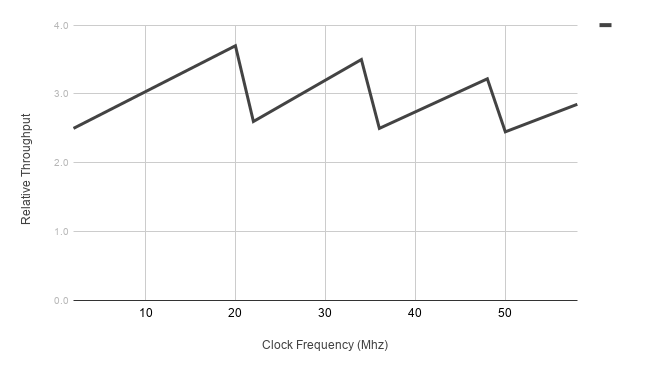
\includegraphics[width=\linewidth]{./figures/throughput_vs_freq_chart1.png}
	\caption{Throughput vs. clock frequency of a typical single-processor system \cite{DBLP:books/daglib/0092408}.}
	\label{fig:troughputvsfreq}
\end{figure}

In a nutshell, while the CPU design evolutionary envolved to serve as a fast instruction worker with lighting reflexes and high clock speeds, DRAM access latency hardly improved over time. This problem can be addressed by applying fast memory to this data processing workflow. But the limitation of data storage is: The faster, the more expensive per capacity it gets and thus smaller. The principle of deviding the memory space into a faster and slower section was already used in the \textit{virtual memory system}. The operating system copies portions of code from the slower to the faster portion to ensure that a high amount of the program-code executes from a very fast memory and resides in slower, less expensive memory when it is waiting to be used \cite{DBLP:books/daglib/0092408}. 

The discovery of the locality principle led to the invention of working-sets \cite{DBLP:reference/db/2009} to make use of locality properties that predict upcoming data references and later enabled the design of page replacement algorithms. A processor caches work quite similar with the difference that their contents are completely controlled by hardware logic.  

\subsection{Cache Hierarchy}

Modern CPU architectures have a hierarchical cache memory structure. It again has economical reasons similar to the difference between DRAM and mass storage devices (e.g.: Hard Disk Drive, Solid State Disk) in virtual memory management. To narrow the exponentially growing performance gap between CPU speed and memory latency, the CPU is composed of multiple ALUs (Arithmetic Logic Units) and lots of hierarchical fast cache memory banks. The speed of the banks increases with less distance to an ALU (core) and decreases when the distance gets bigger. So in fact, processor caches are designed to bridge the gap between the processing speed of a modern processor and the data retrieval speed of the systems main memory in the most economic way possible. 

Cache memory hierarchies exploit the principle of locality and focus on referencing only small fractions for given periods of time. Consequently, during each period of time, only the fraction currently referenced, called working-set, needs to be present in the fastest memory level, while the remaining data and code can stay in slower levels. In general, all data in one level is also found in all (slower but larger) memory levels below it \cite{DBLP:reference/db/2009}. 

Summing it up, caches store the contents of recently used memory locations, as well as working-sets likely to be required by the CPU and evicts working-sets decided to not be useful anytime soon, usually by variations of an LRU (Least Recently Used) replacement algorithm. Retrieving data from a cache significantely reduces the pressure on the main memory and saves time. 

\begin{figure}[!ht]
	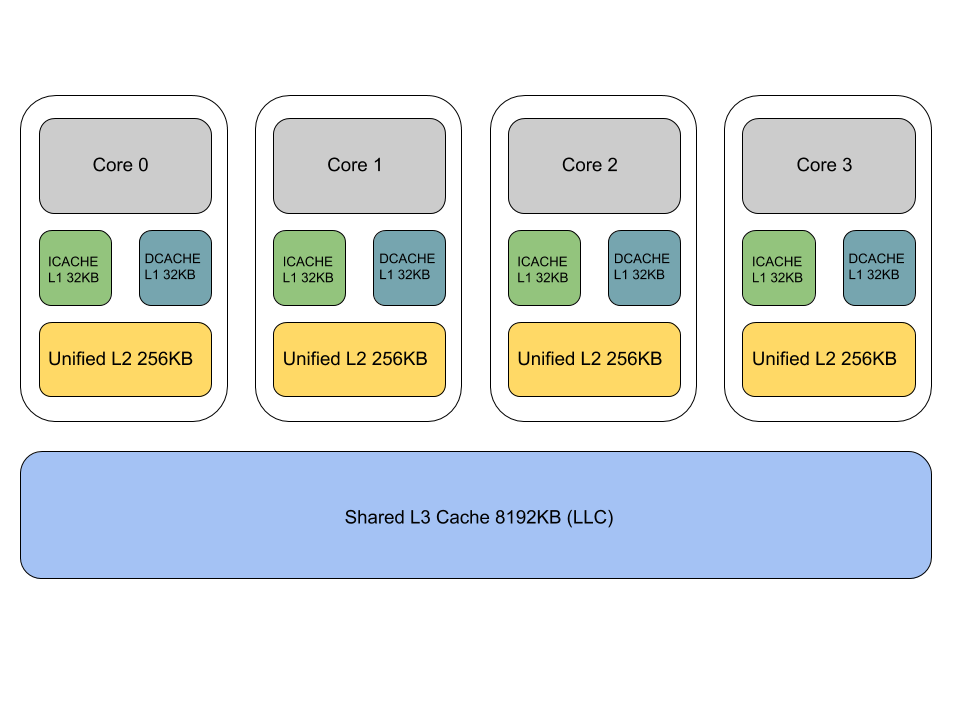
\includegraphics[width=\linewidth]{./figures/multilevel_cache_hierarchy_skylake.png}
	\caption{Multilevel cache architecture (Skylake).}
	\label{fig:cachearchitecture}
\end{figure}

A typical modern processor includes three different cache levels as illustrated in figure \ref{fig:cachearchitecture}, that all rely on the CPU's die. Caches at the top of the hierarchy, typically known as Level 1 or \textit{L1} cache, are the smallest, fastes and nearest to the corresponding processors core. The L1 is split into data and instruction caches on recent Intel processors (32 KiB DCACHE and 32 KiB ICACHE) and has an access time to cached data of 4 CPU cycles. The Level 2 (L2) cache consists of unified data and has a size of 256 KiB and a latency of 7 cycles. In a multicore processor, each of the execution cores has dedicated L1 and L2 caches. The third level cache is called L3 or last-level-cache (LLC). It very much varies between specific processor models. For desktop types the size ranges from 3MiB to 8MiB with a latency of about 35 cycles. Unlike higher-level caches, which are core-private, the LLC is shared between all cores of the processor \cite{DBLP:journals/iacr/YaromGLLH15}. Important is that by definition the LLC contains copies of all the data stored in the lower cache levels as we heard before. That means that deleting data from the LLC also removes this data from all other cache levels. This feature is used by various cache attacks since operating systems offer instructions to manipulate the content of the LLC. 

\subsection{Cache Mapping}

The important characteristics of caches are: \textit{Cache Capacity} (or \textit{Cache Size}), \textit{Cache Lines}, \textit{Block Size} and \textit{Associativity}. A cache stores fixed-size memory units (defined by the block size) called lines to fully fit its capacity. When the processor issues an access to the main memory, the referenced address, also called main memory address or byte address, first gets mapped into the corresponding cache line. In the most simple case of a \textit{direct} mapped cache with a block size of 1 byte, this may be described as: $cache\ line\ index = byte\ address\ mod\ cache\ size$. Instead of performing a division, we can resolve the least significant bits $n$ of a memory address, corresponding to the cache size $2^n$. With a cache size of $2^2$ bytes and a block size of 1 byte, the memory address $14$ maps to cache line with index $2$ that contains a data block of 1 byte. And so would 6: $6\ mod\ 2^2 = 2$. Or by using the 2 least significant bits $01{\underline{10}}_2 = 2_{10}$. Note that we are mapping bytewise right now and therefore $\#cache\ blocks == \#cache\ lines$. 

\textit{Spatial locality} predicts that an access to one memory address will then be followed by an access to a nearby address. A one byte block size don't takes advantage of this observation, so much bigger block sizes are used in practice which oviously changes the mapping. The most common block size nowadays is $2^6 = 64$ bytes. With a block size of $2^k$ bytes we can conceptually split the main memory into $2^k$ byte chunks. We first need to determine a so called \textit{block address}. This can be done with an integer divison like so: $cache\ block\ address = byte\ address\ /\ 2^k$. E.g.: with a cache size of 8 bytes, a block size of 2 bytes, byte address $14$ and $15$ both map to the cache block $7$. With the calculated block address we can map our block to a corresponding cache line by again performing the division with the number of cache blocks (cache lines) to find the remainder: $7\ mod\ 2^2 = 3$. A requirement for cache size and block size clearly is that both sizes have to be a power of 2. When we access one byte of data in the main memory, we copy the whole calculated block to the cache line to hopefully take advantage of spatial locality. 

\begin{figure}[!ht]
	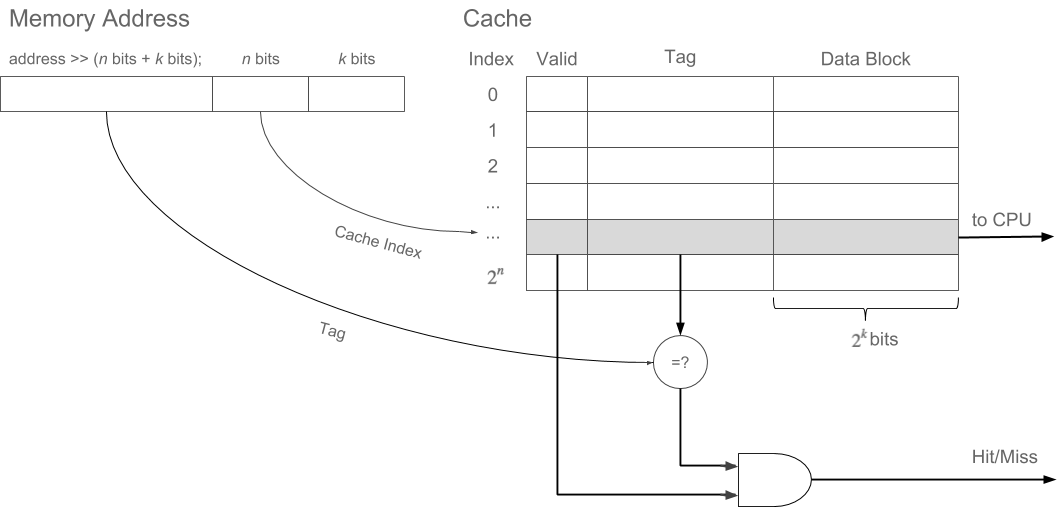
\includegraphics[width=\linewidth]{./figures/direct_cache_mapping.png}
	\caption{Direct cache address resolution.}
	\label{fig:directcache}
\end{figure}

To now locate a specific byte of data in the cache we resolve the byte address as shown in figure \ref{fig:directcache}. Instead of performing divisions we use the least significant $k$ bits as a block offset and $n$ bits to determine the cache line index. %the Relation.. better here? *todo*

This mapping scheme causes that more than one main memory address now map to the same cache line due to the fact that the CPU cache is smaller than the main memory. Therefore a unique identifier called \textit{tag} is introduced. Its the remaining bits of the memory byte address (where $>>$ is bit-wise right shift):  

\begin{verbatim}
tag = address >> (nbits + kbits);
\end{verbatim} 
%after excluding the $n$ and $k$ bits that are used for mapping, 

Tags distinguish between different memory locations that map to the same cache line. We can always match a memory address tag with the content of the mapped cache line to verify if the current block actually present in the cache line is correct for the actual memory access. Additionally a \textit{valid bit} is initialized with zero, when the cache is empty and set when data is loaded into a particular cache line, to determine if the information also is valid at the time. 

The processor always accesses memory for instance to fetch new instructions or load and store data in main memory while executing them. When we use a cache mapping of this form, one of several situations can occur. If the mapped cache line contains invalid data, pointed out by a valid bit, the memory content needs to be loaded from main memory since the cache doesn't contain it. Similarly, if the cache tag fails to match the actual address tag, altough it might be valid information indicated by the valid bit, the requested content needs to be loaded from main memory too, since it holds some data we are currently not looking for. In both of these two cases requested data had to be fetched from main memory, because the cache was not able to provide the information. Either of these two cases is called a \textit{cache miss} \cite{DBLP:journals/iacr/Page02}. The other case is called a \textit{cache hit}. It is signalled when a cache line contains valid content with matching tags that is requested by the processor. In this case the information can be gathered completely through the cache memory without resorting to the slower main memory. 

A direct-mapped cache of this scheme is very easy to compute. Indices and offsets can be computed with bit operators or simple arithmetic as showed above. Every byte address belogs in exactly one block and data gets exchanged by another address on every cache miss. This exploits temporal locality, which assumes that older data is less likely to be requested than newer data. Basically it is a \textit{LRU} (Least Recently Used) replacement algorithm. The whole concept of locality, spatial and temporal, means that the overall time needed to transfer information from one place to another is accelerated because it's likely that cache hits happen more often than cache misses, hence fast memory accesses oudto slower ones resulting in an overall system performance improvement. 
Altough this cache organization causes the least overhead in determining the cache line candidate, it also offers the least flexibility and may cause a lot of conflict misses \cite{DBLP:reference/db/2009}. In practice, memory blocks that belong to the same cache block are often used concurrently. Directly mapped, they always get exchanged with each other and this causes high amount data transfer and importantly a lot of time.  

Today, most architectures employ \textit{set-associative caches}. This means that the cache now is divided into multiple \textit{cache sets} where each set consists of several cache lines (also called \textit{Ways}). Just like before, it depends on the memory address to which cache set the memory block is loaded in the first place. A-way set associative caches allow loading a line in A different positions. A 2-way example is illustrated in figure \ref{fig:associativecache}. In this example 2 cache lines are part of one cache set. On one side it reduces the number of indices, on the other increases the number of possible cache lines, where a particular memory block may be stored in the cache. 

\begin{figure}[!ht]
	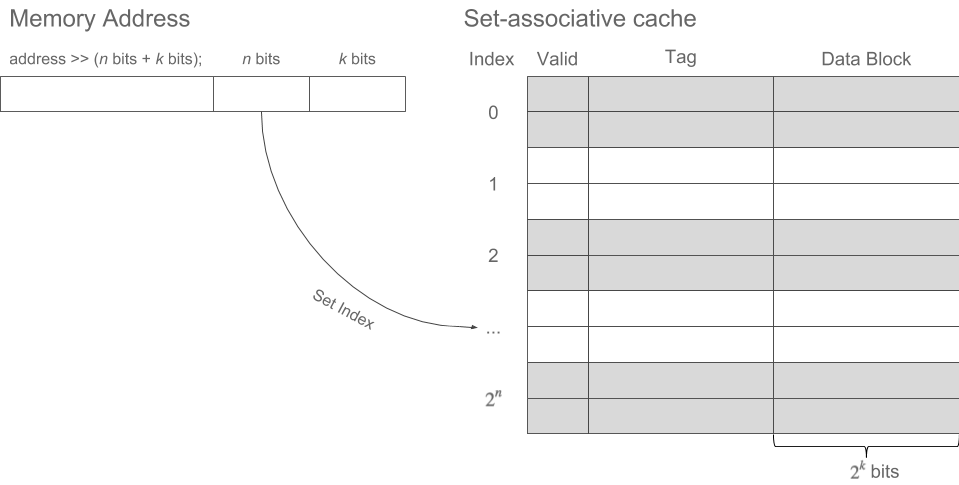
\includegraphics[width=\linewidth]{./figures/a-way-set-associative.png}
	\caption{Assosiative cache principle.}
	\label{fig:associativecache}
\end{figure}

Instead of forcing each memory address into one particular block a set-associative cache permits data to be stored in any cache block that is part of the current set the address is mapped to. Following this principle there is less conflict between two or more memory addresses that map to a single cache line. One price of associativity is the higher effort to find the correct block in the cache. For every memory access we need to compare the tag with all  the tags of A-ways. But this behaviour provides a lot of flexibility in terms of utilizing the principle of temporal locality. If we need to replace a cache line during a cache miss and if A > 1, some smart cache replacement policy determines one from among the A candidates. Least Recently Used (LRU) is the most common replacement algorithm to fullfill this operation. They are much more complex and optimized in comparison with a simple direct-mapped LRU on how to decide what line gets evicted. If A = 1, the cache is called directly-mapped \cite{DBLP:reference/db/2009}.

Following the principle of virtual memory management \cite{DBLP:books/lib/Tanenbaum09}, for data access, logical virtual memory addresses used by application code have to be translated to physical page addresses in the main memory. The \textit{Translation Lookaside Buffer} (TLB) is used as a cache for physical page addresses, holding the translation for the most recently used pages. If a virtual address is found in this cache, the translation to a physical address has no additional cost \cite{DBLP:reference/db/2009}. As a consequence of this virtual memory management we need to distinguish between virtually indexed and physically indexed caches. In general, virtually indexed caches are considered to be faster than physically indexed caches \cite{DBLP:conf/uss/GrussSM15}. An advantage of virtually indexed caches is, that the cache line can be looked up in parallel with the translation of the virtual address done by the TLB. Different virtual addresses mapping to the same physical address may be cached in different cache lines in virtually indexed caches. Tags help in order to uniquely identify a specific cache line within a cache set, but even tags can either be virtually or physically. Summarized, caches are grouped as follows: \textit{Physically indexed, physically tagged - Virtually indexed, virtually tagged - Virtually indexed, physically tagged - Physically indexed, virtually tagged}. So this is based on wheter the index or tag correspond to virtual or physical addresses. However, within a modern computer system different types of caches are used and combined, each having advantages and disadvantages in comparison beneath each other. 

Since the Sandy Bridge microarchitecture, Intel introduced a new design for the last-level cache

The 3rd-level cache is organized as multiple cache slices, the size of each
slice may depend on product configurations, connected by a ring interconnect. %Intel paper 2452

\subsection{Page Sharing}
\subsection{Cache Attacks}
\subsection{Qemu}

\subsection{MY WORK SOMETHING}

Data can be speculatively loaded to the L1 DCache using software prefetching, hardware prefetching, or
any combination of the two. % INTEL PAPER 2.4.5.4

direct:
The relation $cache\ capacity\ /\ cache\ block\ size$ returns the amount of cache lines needed for this particular cache and block size. To calculate the number of bits needed for the block offset as well as cache index, we use the definition of the logarithm: $x = log_a (y) \equiv y = a^x$. To be able to map every cache line we caclulate the number of $n$ bits with $log(cache\ lines) / log(2)$ and to address each and every byte in a cache line the number of $k$ bits with $log(block\ size) / log(2)$. 


ass:
 The number of $n$ bits can now be calculated with $log(cache\ size) / ways) / log(2)$. 
 
 
\section{Conclusion}
\label{conclusion}
Write conclusion

\onecolumn
\pagebreak
\twocolumn
\bibliographystyle{plain}
\bibliography{bibliography}
%\nocite{*}
\end{document}
